\chapter{Virtuelle Private Netzwerke}

Der Zugriff aus der Ferne auf das lokale Firmennetzwerk ist für verschiedene Anwendungsszenarien unabdingbar. Die Vernetzung von Firmenstandorten, der Zugriff von mobilen Mitarbeitern auf das Firmennetz oder auch ein Zugang für Geschäftspartner auf das Intranet des Unternehmens müssen sicher Umgesetzt werden.
Die Technologie, die dies ermöglichen soll ist \emph{VPN}. Ein VPN ist ein virtuelles privates Netz, eine logische Verbindung die auf einem anderen, physischen Netz aufgebaut wird \cite{zisler2018computer}. Grundsätzlich eignet sich jedes Netz, hier wird jedoch nur die Verwirklichung von VPN über das Internet betrachtet. Es wird unter anderem wird zwischen folgenden Varianten unterschieden:
\begin{itemize}
  \item Site-to-Site/ Branch Office VPN: Verbindung von verschiedenen Firmenstandorten,
  \item End-to-Site/ Remote Access VPN: Verbindung eines Heimarbeitsplatzes oder eines Mobilen Mitarbeiters it dem Intranet des Unternehmens.
  \item End-toEnd VPN: Verbindung zweier Endgeräte,
  \item Extranet VPN: gewährt einem Geschäftspartner/Kunden/Lieferanten Zugang zu Teilen des Internen Netzes 
\end{itemize}

Die Umsetzung des VPN kann entweder bei einem Dienstleister eingekauft werden, dies nennt sich \emph{Trusted VPN}, oder selber als \emph{secure VPN} aufgebaut werden. Beim Einsatz von Trusted VPN sollten vertrauliche Daten zusätzlich auf Anwendungsebene verschlüsselt werden, um sie zum Beispiel vor Innentätern des Dienstleisters zu schützen. 
 Es gibt außerdem Zwischenformen, so dass nur Teile der Technologie bei einem Dienstleister eingekauft werden.


\section{Funktionsweise}

Die Basistechnologie die einem VPN zugrundeliegt ist das \emph{Tunneling}. Es handelt sich um ein Verfahren, welches  Netzwerkprotokolle in beliebige andere Netzwerkprotokolle kapselt. 




\section{Architektur}
Das VPN-Gateway kann an verschieden Stellen an das Netzwerk angeschlossen werden. Zu beachten ist

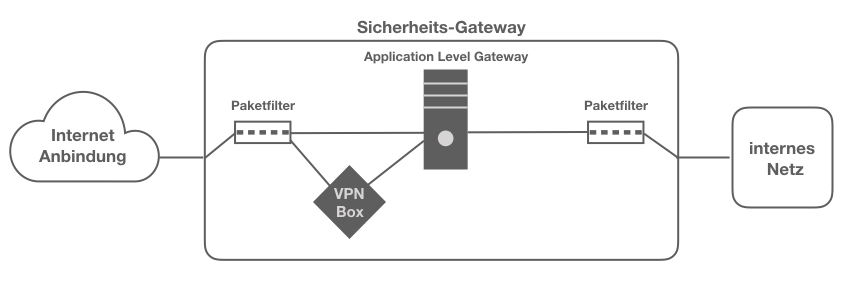
\includegraphics[width=\linewidth]{vpnarchitektur.jpeg}

\section{Anwendungsbereiche in privaten Haushalten}

Virtuelle private Netzwerke werden auch im privaten Bereich  verwendet. Hier gibt es hauptsächlich zwei Anwendungsszenarien: der Zugriff aus der Ferne auf das Heimnetzwerk zur Bedienung des IoT (Internet of Things) oder der Zugriff auf die NAS als Cloud-Alternaive oder






